\documentclass[border=12pt]{standalone}
\usepackage{tikz}
\usetikzlibrary{shapes.geometric, arrows.meta, positioning, calc, fit, backgrounds}
\usepackage{fontspec}
\setmainfont{DejaVu Sans}

\begin{document}
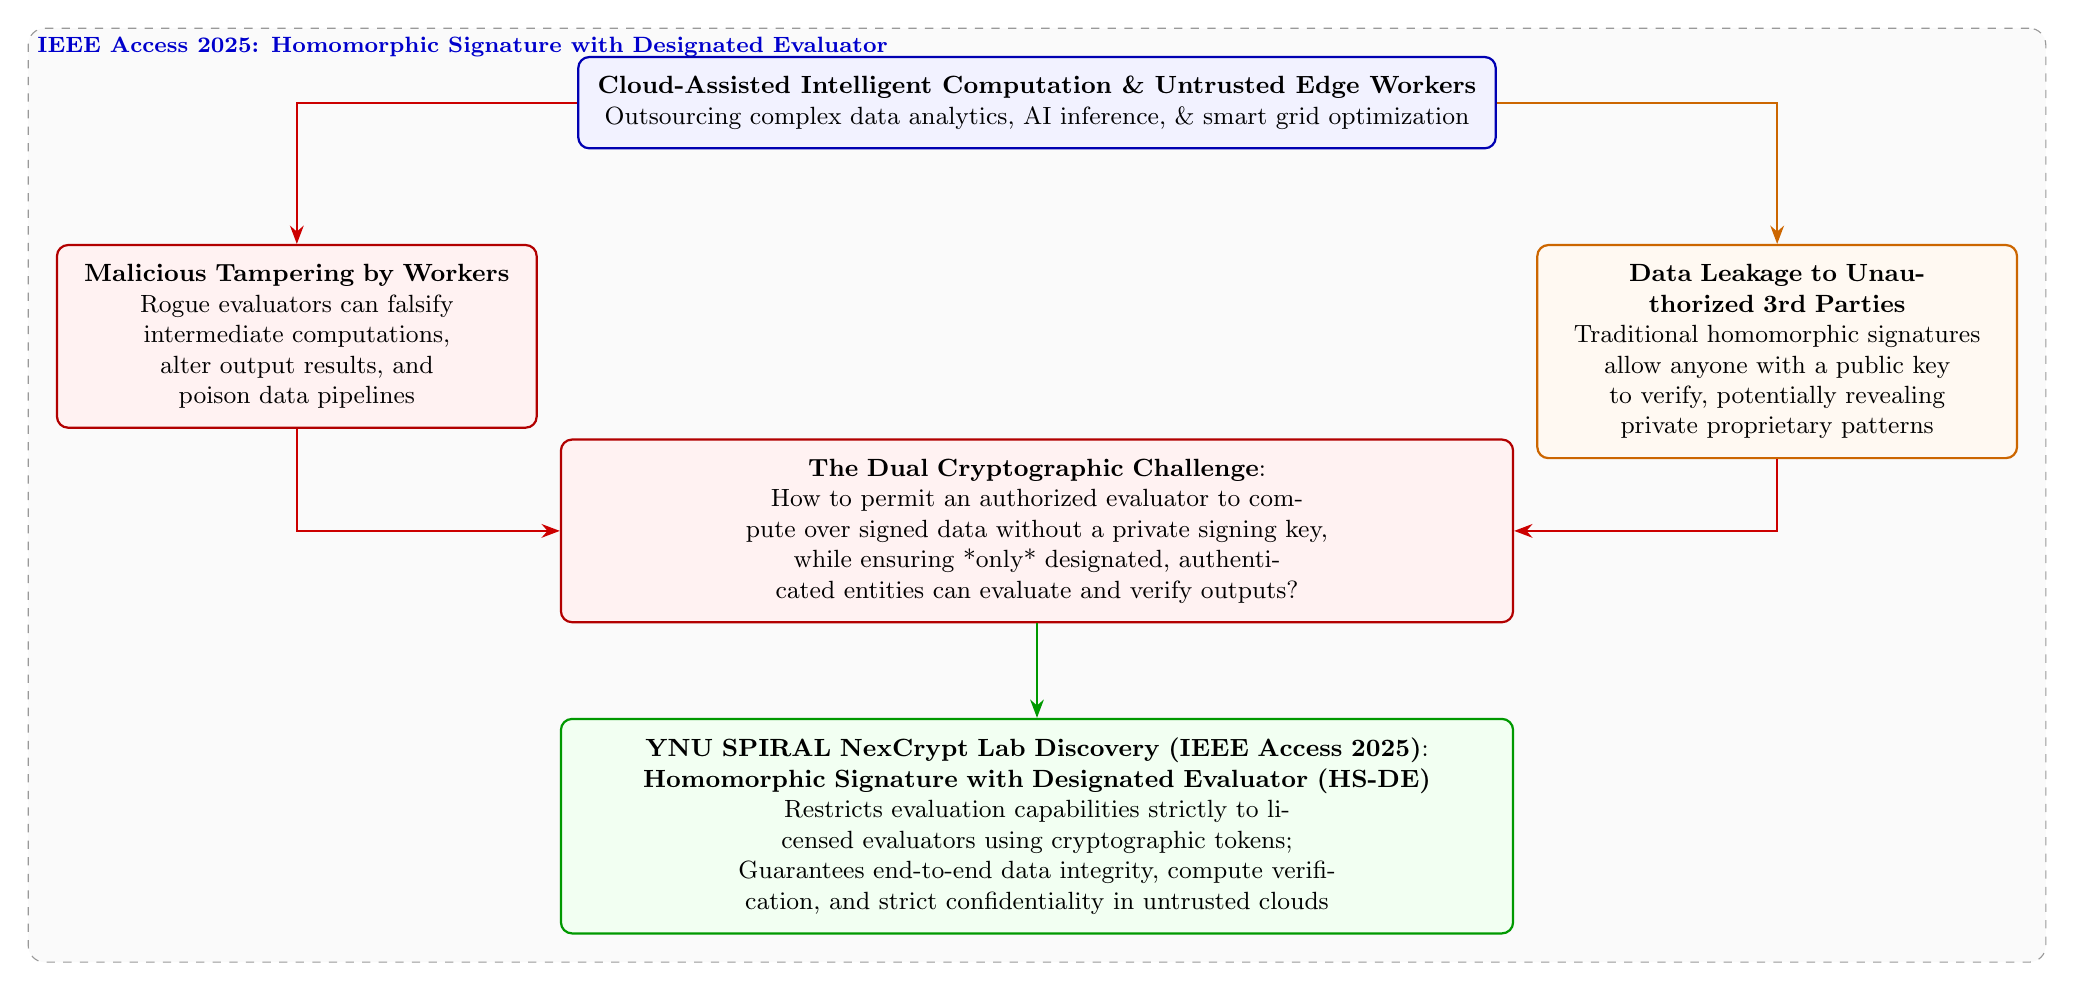
\begin{tikzpicture}[
    font=\small,
    >=Stealth,
    node distance=1.2cm,
    block/.style={rectangle, draw=blue!70!black, fill=blue!5, rounded corners=4pt, thick, align=center, inner sep=7pt},
    alertblock/.style={rectangle, draw=red!70!black, fill=red!5, rounded corners=4pt, thick, align=center, inner sep=7pt},
    greenblock/.style={rectangle, draw=green!60!black, fill=green!5, rounded corners=4pt, thick, align=center, inner sep=7pt},
    amberblock/.style={rectangle, draw=orange!80!black, fill=orange!5, rounded corners=4pt, thick, align=center, inner sep=7pt},
    groupbox/.style={draw=black!40, dashed, rounded corners=6pt, fill=black!2, inner sep=10pt}
]

    % Top Concept
    \node[block] (cloud) {\textbf{Cloud-Assisted Intelligent Computation \& Untrusted Edge Workers}\\Outsourcing complex data analytics, AI inference, \& smart grid optimization};

    % Two Threat Pillars in Standard Signatures
    \node[alertblock, below left=1.2cm and 0.5cm of cloud, text width=5.6cm] (forgery) {\textbf{Malicious Tampering by Workers}\\Rogue evaluators can falsify intermediate computations,\\alter output results, and poison data pipelines};

    \node[amberblock, below right=1.2cm and 0.5cm of cloud, text width=5.6cm] (leakage) {\textbf{Data Leakage to Unauthorized 3rd Parties}\\Traditional homomorphic signatures allow anyone with a public key\\to verify, potentially revealing private proprietary patterns};

    \draw[->, thick, red!80!black] (cloud) -| (forgery);
    \draw[->, thick, orange!80!black] (cloud) -| (leakage);

    % Challenge
    \node[alertblock, below=1.2cm of $(forgery)!0.5!(leakage)$, text width=11.6cm] (challenge) {\textbf{The Dual Cryptographic Challenge}:\\How to permit an authorized evaluator to compute over signed data without a private signing key,\\while ensuring *only* designated, authenticated entities can evaluate and verify outputs?};

    \draw[->, thick, red!80!black] (forgery) |- (challenge);
    \draw[->, thick, red!80!black] (leakage) |- (challenge);

    % Solution: YNU NexCrypt IEEE Access 2025 Study
    \node[greenblock, below=1.2cm of challenge, text width=11.6cm] (solution) {\textbf{YNU SPIRAL NexCrypt Lab Discovery (IEEE Access 2025)}:\\\textbf{Homomorphic Signature with Designated Evaluator (HS-DE)}\\Restricts evaluation capabilities strictly to licensed evaluators using cryptographic tokens;\\Guarantees end-to-end data integrity, compute verification, and strict confidentiality in untrusted clouds};

    \draw[->, thick, green!60!black] (challenge) -- (solution);

    \begin{scope}[on background layer]
        \node[groupbox, fit=(cloud) (forgery) (leakage) (challenge) (solution), label={[anchor=north west, font=\footnotesize\bfseries, blue!80!black]north west:IEEE Access 2025: Homomorphic Signature with Designated Evaluator}] {};
    \end{scope}

\end{tikzpicture}
\end{document}
